%!TEX root = ../main.tex

\graphicspath{{./figures/chapter4/}}


\chapter{Spatial feature engineering} \label{ch:chapter4}
\minitoc
\newpage

In this chapter we present and discuss different approaches to analyze \ac{RNA} localization patterns.
They require to quantify and measure indicators from fluorescent images.
To do so, we use a coordinate representation of cells, merging results from the detection~\ref{ch:chapter2} and segmentation~\ref{ch:chapter3} chapters.

We first present this representation, obtained with methods implemented in \emph{bigfish.multitask}.
In the second and third parts of this chapter we then present two different methods to compute spatial features.
We can manually design localization features or we can learn them, training a gradient-based pipeline on a pretext task.

The hand-crafted features are already implemented in \emph{bigfish.classification}.
The learned features section was mainly developed with the paper:

\begin{center}
	\color{green}
	Future paper to be released (ECCV workshop or arxiv)
\end{center}

\section{From images to coordinates} \label{sec:image_coordinates}

We mainly base our analysis on the coordinate representation of cells as illustrated in figure~\ref{fig:cell_extracted_0}.
We exploit outcomes from detection and segmentation stages.
More precisely, we extract and identify for each individual cell coordinates of detected objects and segmentation masks.
As a reminder, current implementation in \emph{bigfish} allows a 2D or 3D detection, but only a 2D segmentation.
However, any external methods could be used, as long as output format fits.

\begin{figure}[h]
    \centering
    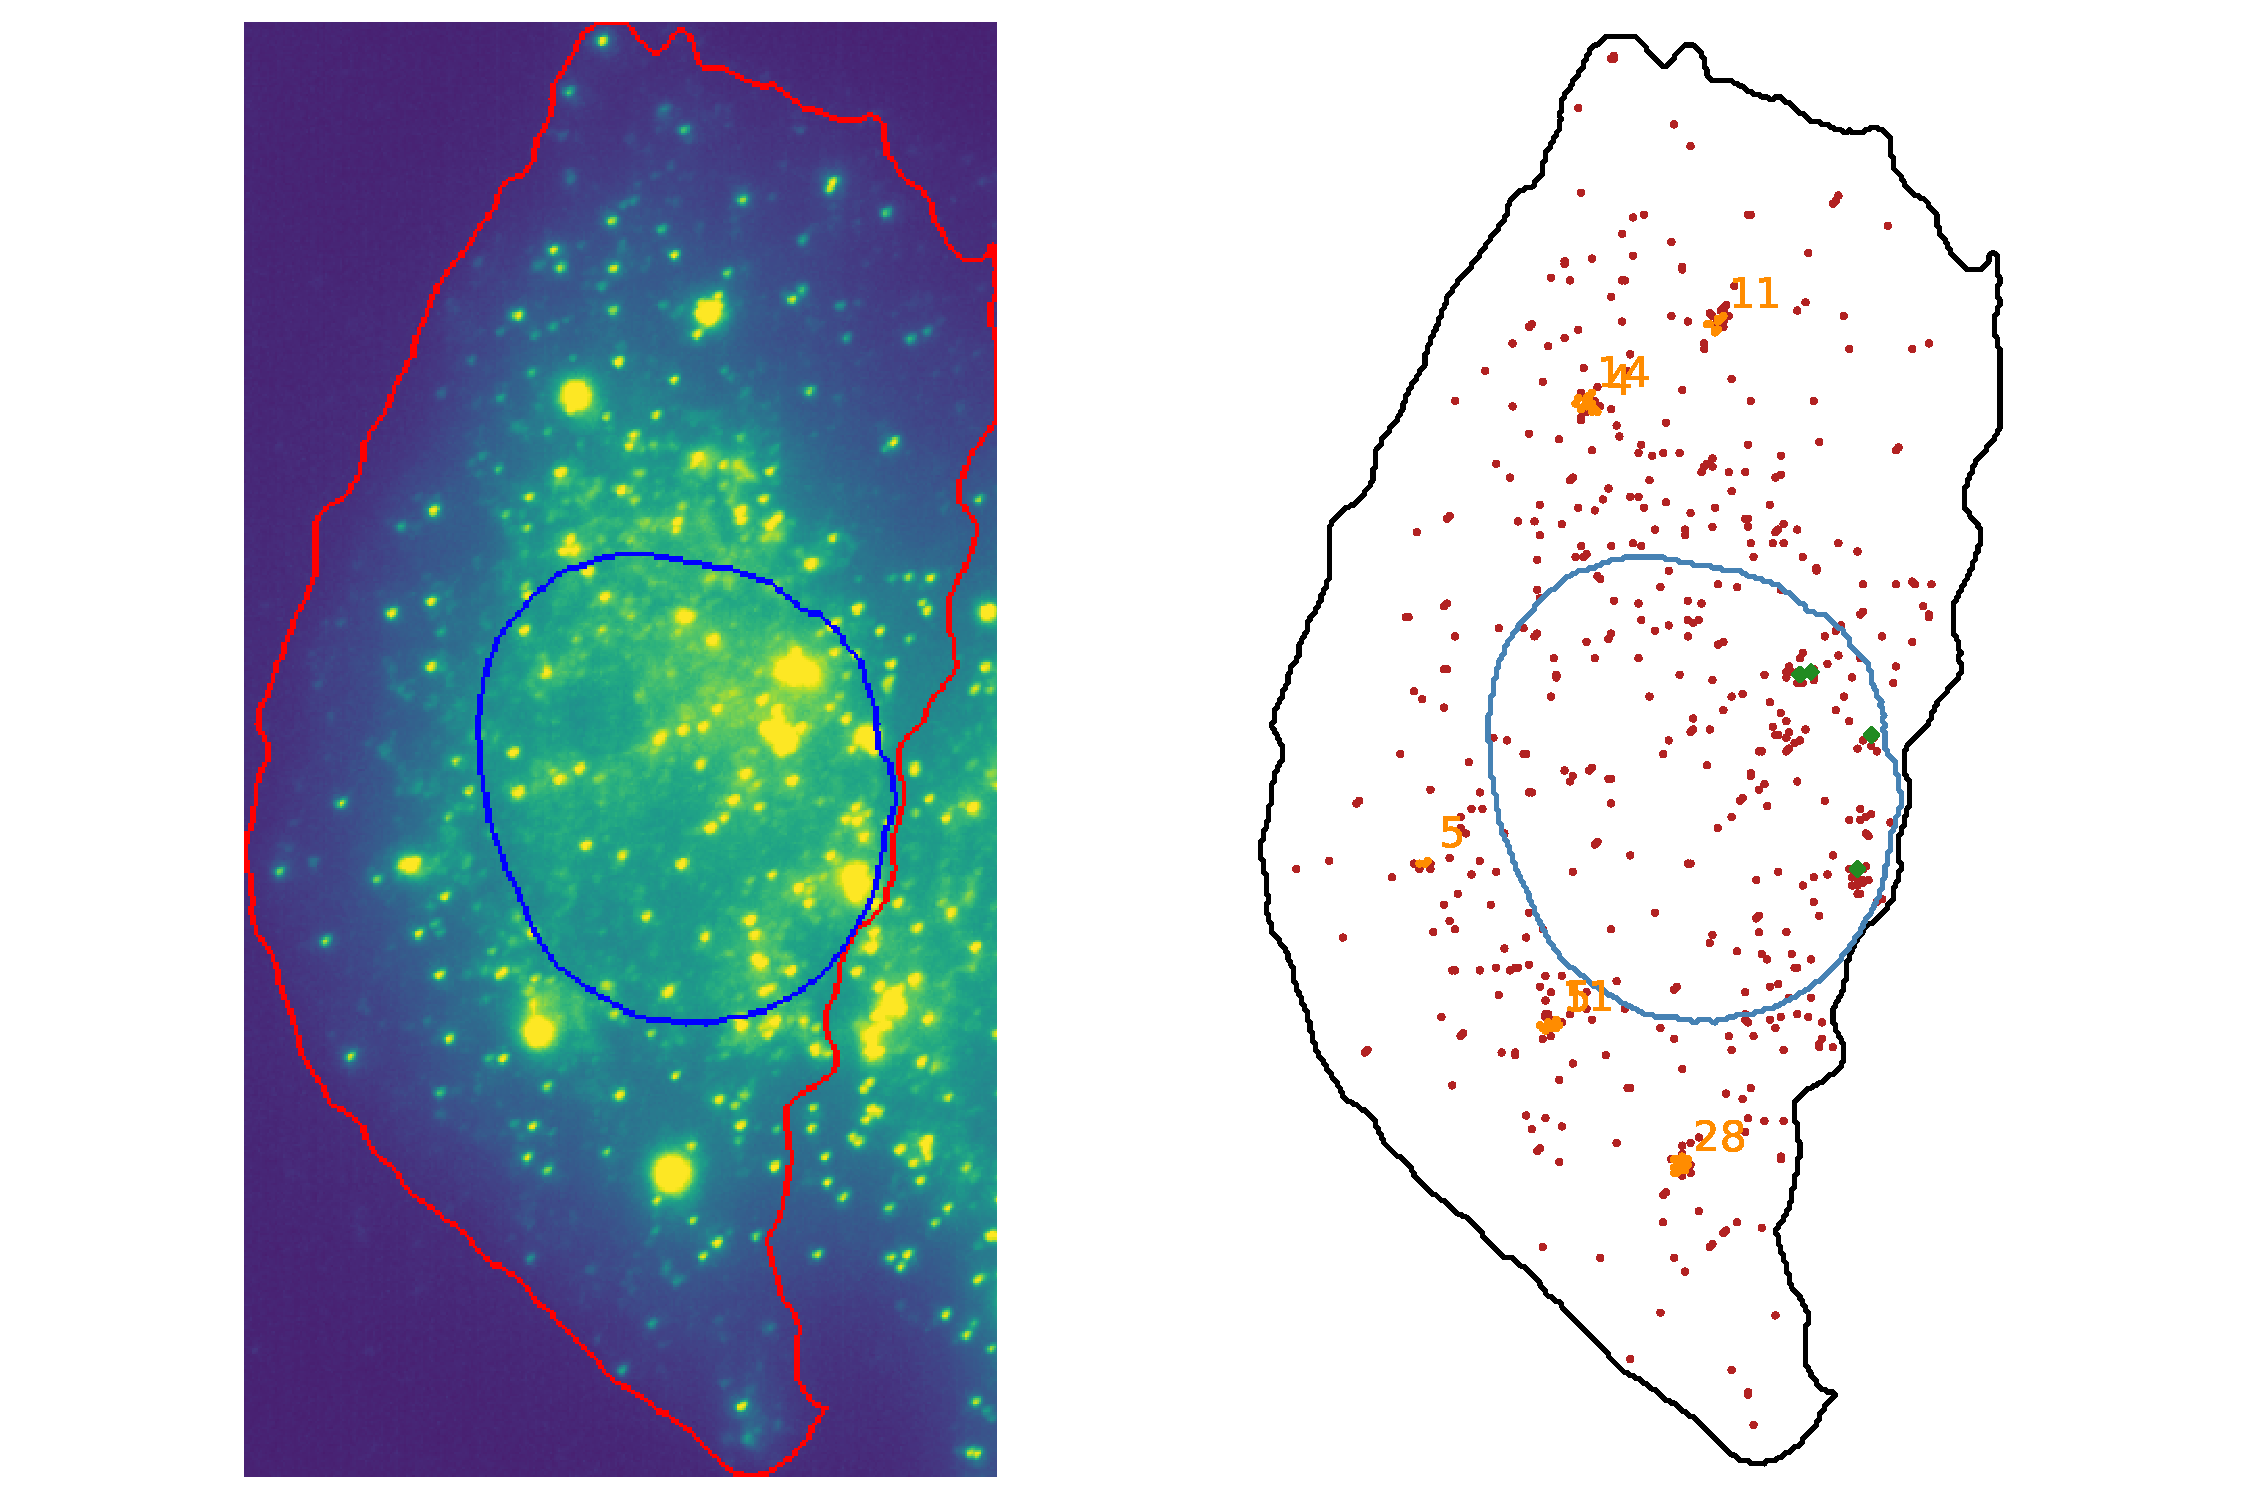
\includegraphics[width=1\textwidth]{figures/chapter4/cell_extracted_0}
    \caption{Original image (left) and coordinate representation (right)}
    \label{fig:cell_extracted_0}
\end{figure}

\paragraph{Detected object labelling}

In addition to detection and segmentation refinement, the possibility to merge results from both stages is highly valuable.
We can discriminate individual objects according to their localization in the cell.
A user might want to label a detected object if it locates within a segmented surface or not.
For example, some studies require to remove transcription sites before further analysis~\cite{CHOUAIB_2020}, or on the contrary to focus on them.
User could define a \ac{RNA} cluster inside nucleus as a transcription site, as opposed to the ones detected outside nucleus.
More generally, any detected object could be assigned to a specific cellular compartments, depending on the fluorescent labels available in the study.\\

% reference paper using transcription site only

\begin{minipage}{0.9\textwidth}
\begin{lstlisting}[language=Python]
import bigfish.multistack as multistack

# discriminate foci and transcription sites
spots_no_ts, foci, ts = multistack.remove_transcription_site(
	rna=spots,
	clusters=clusters,
	nuc_mask=nuc_label,
	ndim=3)
\end{lstlisting}
\end{minipage}

\paragraph{Cell extraction}

To extract and summarize our \ac{FISH} results at the single cell level, the only requirement is a segmentation mask of the cell.
At least, user needs to perform instance segmentation to be able to identify individual cells.
Additional results are optional, but they greatly improve the quality of the information assigned to each cell.
Detected \ac{RNA} and cluster (or anything else detected) can be assigned to individual cells.
Nuclei segmentation masks make us able to delimitate nuclear membrane and define transcription sites or any nucleus-related object.
We can also crop input images around the identified cells, for every available channels.

In figure~\ref{fig:cell_extracted_0} we can observe a cropped \ac{smFISH} image on the left, with cell and nuclear membranes in red and blue respectively.
On the right, these membranes are also visible (in black and blue respectively), in addition with \ac{RNA} spots (in red), \ac{RNA} clusters (in orange, with the estimated number of \ac{RNA} clustered) and transcription sites (in green).
With such \emph{extraction} we lose pixel-wise information like intensity values or image texture.
We also deeply rely on detection and segmentation performances to return meaningful coordinates.
Nonetheless, coordinate representation is a sparse and more natural representation for \ac{mRNA} localization pattern classification.
Indeed \ac{mRNA} molecules can be viewed as single point objects distributed in a 3D space.
Microscopic images with fluorescent labels are here the only medium we have to measure and approximate their localization.

Eventually we propose optional criteria to identify individual cells and refine the outcome.
First, we can ensure that only one nucleus is assigned to each cell.
Second, we can remove cropped cells at the border of the \ac{FoV}.
Their segmentation is incomplete and might bias final results.
Third, extracted cells can be filtered out according to the number of detected objects (especially the number of \ac{RNA}).
By censoring empty cells, we remove potential outliers, detection or segmentation failures and therefore help a subsequent statistical analysis.\\

\begin{minipage}{0.9\textwidth}
\begin{lstlisting}[language=Python]
import bigfish.multistack as multistack

# extract cell-level results
fov_results = multistack.extract_cell(
    cell_label=cell_label,
    ndim=3,
    nuc_label=nuc_label,
    rna_coord=spots_no_ts,
    others_coord={"foci": foci, "transcription_site": ts},
    image=image_contrasted,
    others_image={"dapi": nuc_mip, "smfish": smfish_mip})
\end{lstlisting}
\end{minipage}

\paragraph{Statistical description}

At this stage we can already compute standard, but useful statistics for every cells.
We measure cell and nucleus areas, but also \ac{RNA} distribution, inside and outside nucleus.
With cluster coordinates, estimation of cluster size is available, as well as proportion of clustered \ac{RNA}.
The \ac{RNA} proportion in specific cellular compartments are also noteworthy.
Such indicators are already relevant to quantify or validate meaningful biological insights.
For example, a recent study~\cite{cochard_rna_2022} use \emph{bigfish} to estimate \ac{RNA} recruitment in bioengineered condensates (segmented from a \ac{GFP} channel).\\

\begin{minipage}{0.9\textwidth}
\begin{lstlisting}[language=Python]
import bigfish.multistack as multistack

# compute cell-level statistics
df = multistack.summarize_extraction_results(fov_results, ndim=3)
\end{lstlisting}
\end{minipage}

\section{Hand-crafted localization features} \label{sec:hand_features}

% intro subsections

\subsection{Related work} \label{subsec:related_work_hand_features}

% reference classical fish analysis (battich + stoegger)
% reference dypfish
% reference spatial statistics (carolina whelbi)

\subsection{Expert features} \label{subsec:expert_features}

% input preparation
% distance features
% dispersion features
% morphological features
% centrosomal features
% (plot boxplot)
% (plot RDI or opening)

Feature engineering Aubin designed features from the cloud point representation
of the cell in order to discriminate the different localization patterns. He
gathered more than 20 features in a tabular format
(one row per cell), ready to feed a machine learning model.
A first set of features is based on the euclidean distance. We compute the distance between each
mRNAs and the centroid of the cell, the centroid of the nucleus, the cell border and
the nucleus border. Averages and quantiles are then computed from these distances and finally normalized.
A second set of features involved the Ripley K-function. It quantifies the aggregation or dispersion of mRNAs:
K(r)=1∑n Npi(r) (7) nλ
i=1
with r the distance range, Npi (r) the number of mRNAs in a circle of radius r centered
on the ith mRNA and λ the total density of mRNAs in the cell (the total number of mRNAs
normalized by the cell area). Several features are returned from this function like the
maximum values, the Spearman correlation with the radius r, etc... Such features are
useful to discriminate foci patterns. A corrected version of the function is actually
used, less sensitive to boundary effects (mRNAs close to a border have a limited neighbourhood).
A third set of features is based on morphological opening (an erosion followed by a dilation).
Applying openings with different sizes, we remove cell’s extensions. We can count the mRNAs
we loose and compute their proportion with the total number of mRNAs. The idea is to detect
RNA localization in cell extensions.
A final group of features concern the proportion of mRNAs inside the nucleus, a dispersion
and a polarization index.

% reference FQ1 (aubin)
% reference rdi calculator

%\paragraph{}


Here, we list the different spatial features that are implemented in big-fish and permit a classification of cells based on their RNA localization patterns. Features are grouped into different classes.
Feature
Description
Area of nucleus
Measured in pixels.
Area of cell
Measured in pixels.
Area of cell extension
The cell area removed by an opening of size 3000nm (an erosion followed by a dilation). Measured in pixels.
Proportion of nucleus area
Proportion of the nucleus area compared to the entire cell.
Table S2. Features to describe cell morphology.
Feature
Description
Total number of mRNAs
-
Number of mRNAs inside nucleus
-
Proportion of mRNAs inside nucleus
Proportion of the mRNAs localizing inside the nucleus compared to the total number of mRNAs in the cell.
Proportion of mRNAs in foci
Proportion of mRNAs clustered in a foci compared to the total number of mRNAs in the cell.
Proportion of mRNAs in cell extension
Proportion of mRNAs in cell extension compared to the total number of mRNAs in the cell.
mRNA proportion along nuclear envelope
Proportion of mRNAs within 500 nm from the nuclear envelope compared to the total number of mRNAs in the cell.
Proportion of mRNAs in specific subcellular areas
Proportion of mRNAs in specific subcellular regions compared to the total number of mRNAs. Five concentric regions are defined around the nuclear envelope: 500-1000 nm, 1000-1500 nm, 1500-2000 nm, 2000-2500 nm and 2500-3000 nm. Six concentric regions are defined from the cell membrane: 0-500 nm, 500-1000 nm, 1000-1500 nm, 1500-2000 nm, 2000-2500 nm and 2500-3000 nm.
Polarization index
Measurement of the mRNA point cloud polarization in the cell. The higher the more polarized are the mRNAs. Index is computed based on the distance between the mRNAs centroid and the cell centroid. Details in (6).
Dispersion index
Measurement of the mRNA point cloud dispersion in the cell. The higher the more dispersed are the mRNAs. Details in (6).

Peripheral distribution index
Measurement of how close the mRNAs localize to the cell periphery. Details in (6).
Mean/median mRNA distance to centrosome
Expressed as an index: mean/median distance over the expected mean/median distance if mRNAs were distributed uniformly in the cell.
Proportion of mRNAs around centrosome
Proportion of mRNAs within 2000 nm from a centrosome compared to the total number of mRNAs in the cell.

\begin{figure}[h]
    \centering
    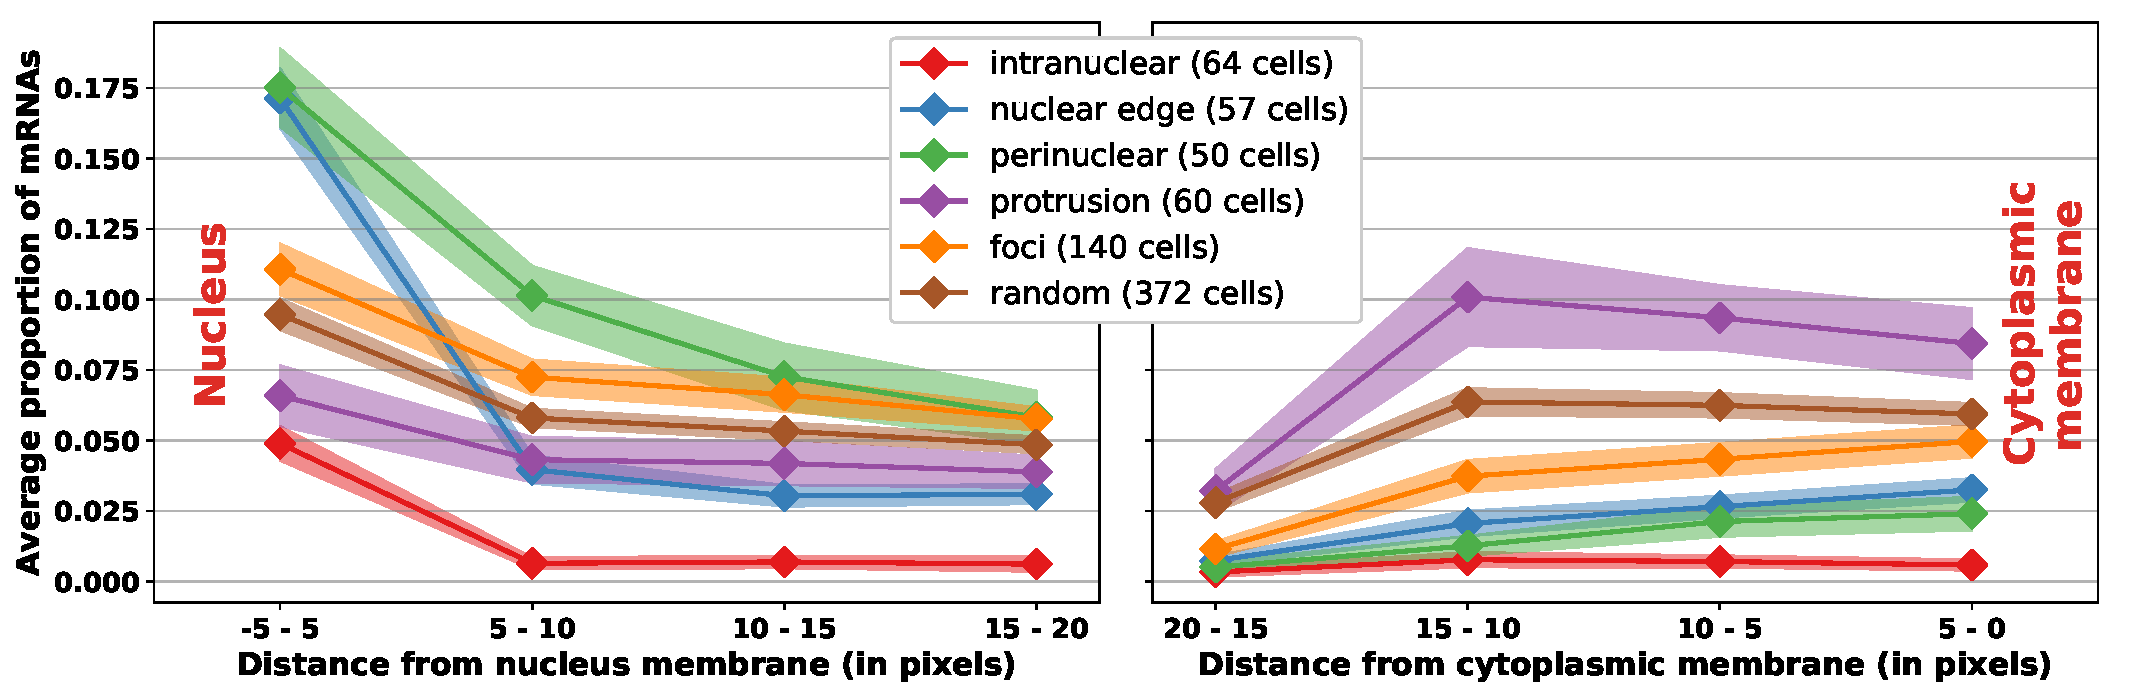
\includegraphics[width=1\textwidth]{figures/chapter4/plot_topography}
    \caption{Concentric distances from cell and nuclear membrane}
    \label{fig:features_topography}
\end{figure}

\begin{wrapfigure}{R}{0.40\textwidth}
  \begin{center}
    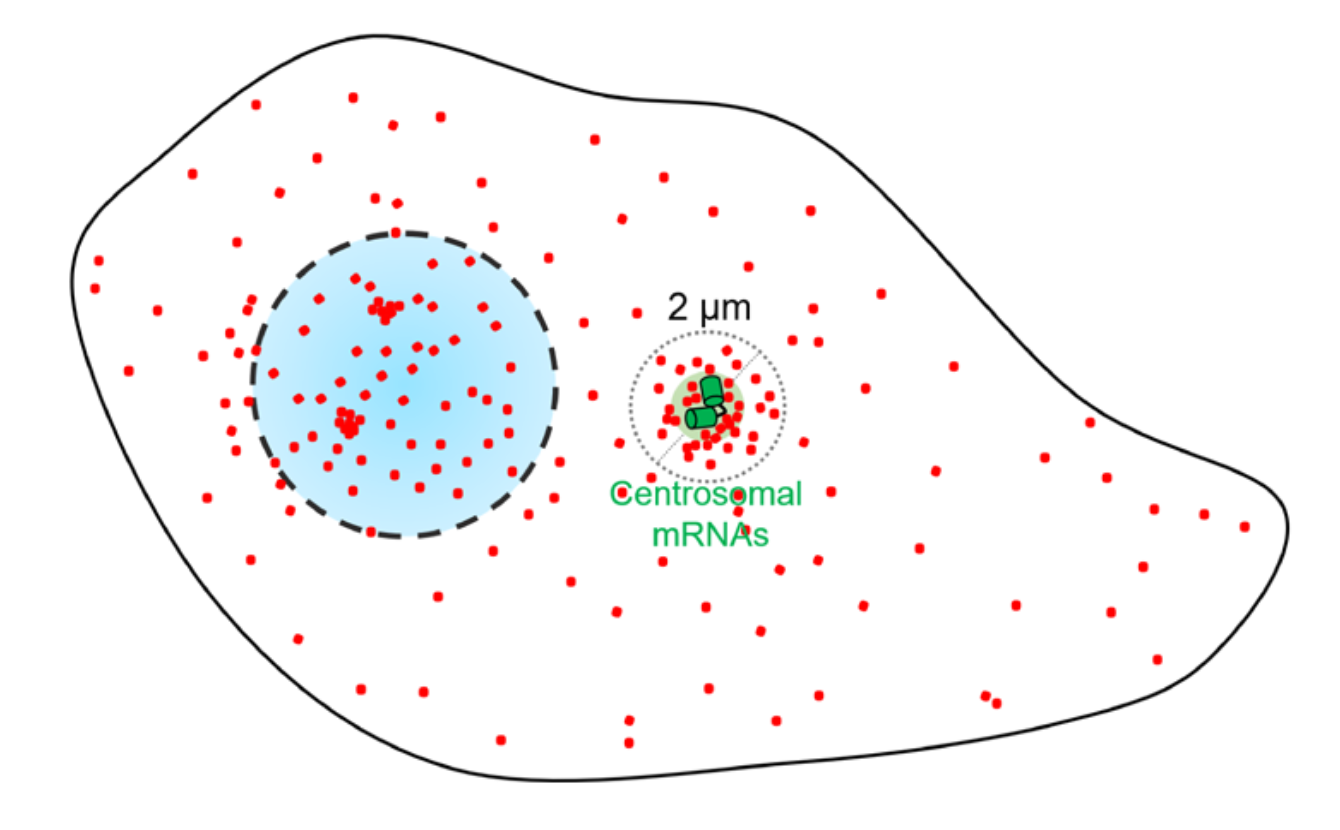
\includegraphics[width=0.33\textwidth]{figures/chapter4/centrosomal_features}
  \end{center}
  \caption{Centrosomal features}
  \label{fig:centrosome_features}
\end{wrapfigure}


\begin{minipage}{0.9\textwidth}
\begin{lstlisting}[language=Python]
import bigfish.classification as classification

# compute features
features, features_names = classification.compute_features(
    cell_mask=cell_mask,  # individual cell mask
	nuc_mask=nuc_mask,  # individual nucleus mask
	ndim=3,
	rna_coord=rna_coord,
    smfish=smfish,
	voxel_size_yx=103,  # in nanometer
    foci_coord=foci_coord,
    compute_distance=True,
    compute_intranuclear=True,
    compute_protrusion=True,
    compute_dispersion=True,
    compute_topography=True,
    compute_foci=True,
    compute_area=True,
    return_names=True)
\end{lstlisting}
\end{minipage}

\section{Learned localization features} \label{sec:learned_features}

% intro subsections

\subsection{Pretext task: simulated pattern classification} \label{subsec:simulation_localization}

% plot simulations
% explain simulations

\begin{figure}[h]
    \centering
    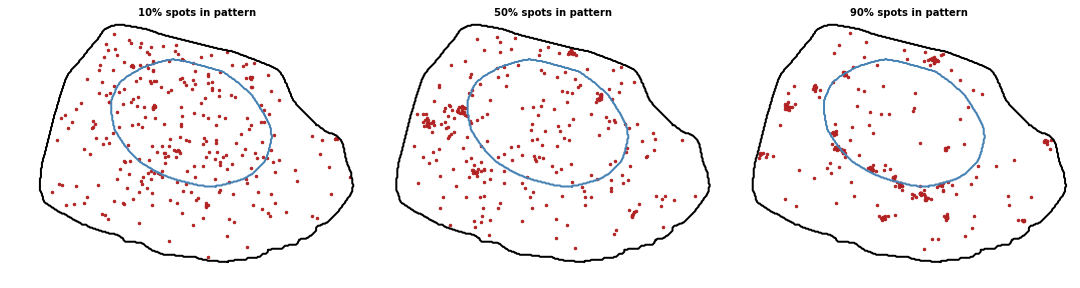
\includegraphics[width=1\textwidth]{figures/chapter4/foci_panel}
    \caption{Foci pattern simulations}
    \label{fig:foci_panel}
\end{figure}

\begin{figure}[h]
    \centering
    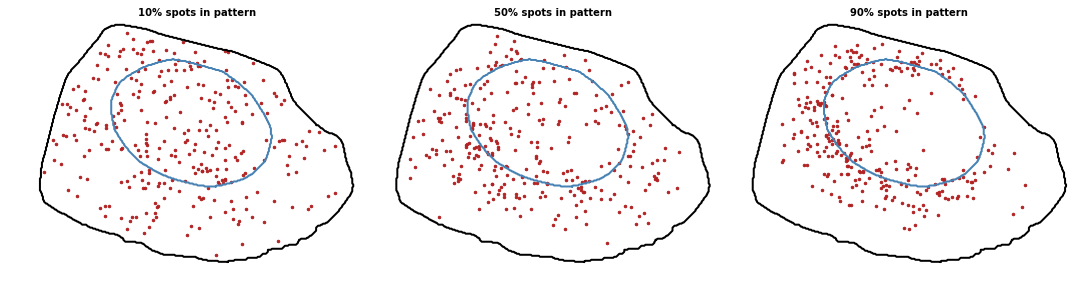
\includegraphics[width=1\textwidth]{figures/chapter4/perinuclear_panel}
    \caption{Perinuclear pattern simulations}
    \label{fig:perinuclear_panel}
\end{figure}

\begin{minipage}{0.9\textwidth}
\begin{lstlisting}[language=Python]
import simfish as sim

# load template dataset
path_template_directory = load_extract_template(path_output)

# localization pattern simulation
instance_coord = sim.simulate_localization_pattern(
	path_template_directory,
	n_spots=150,
	pattern="intranuclear",
	proportion_pattern=0.6)
\end{lstlisting}
\end{minipage}

\subsection{Related work} \label{subsec:related_work_learned_features}

% references neural network to build features
% 3-4 papers cnn features in image
% 3-4 papers cnn features in bioimage
% 3-4 papers cnn features with protein localization
% Bouilohol

% 1-2 paper review (deep laerning with bioimage)
% paper isbi + reference appendix
% 1-2 paper review (deep learning with point cloud)

% transition from cnn to pointcloud (pb localization with cnn // protein localization == texture classification)

% pointnet
% dgcnn
% pointtransformer
% pointmlp

% general review shape classification with point cloud (kernel, curve, pointcnn, voxel3D)

% ML and DL (pointnet) to classify caveolae clusters and non-caveolae clusters
%%~\cite{khater_caveolae_2019}
%% Specifically, we are generating abalanced dataset of 1000 blobs of isotropic
%% point clouds and 1000 blobs of non-isotropic point clouds. The isotropic
%% class of blobs mimicking the caveolae (positive class) and the non-isotropic
%% class mimicking the non-caveolae (negative class). The non-isotropic class of
%% blobs are more planar structures, while the isotropic class are more spherical
%% structures.
%
%% Caveolae are plasma membrane invaginations whose formation requires caveolin-1 (Cav1),
%% the adaptor protein polymerase I,and the transcript release factor (PTRF orCAVIN1).
%% Caveolae have an important role incell functioning, signaling, and disease. Inthe
%% absence ofCAVIN1/PTRF, Cav1 forms non-caveolarmembrane domains called scaffolds.
%% Inthis work, we train machine learning models toautomatically distinguish between
%% caveolae and scaffolds from single molecule localization microscopy (SMLM) data
%% The first uses arandom forest classifier applied to28 hand-crafted/designed features
%% (expert features), the second uses aconvolutional neural net (CNN) applied toaprojection
%% ofthe point clouds onto three planes, and the third uses aPointNet model, a recent
%% development that can directly take point clouds as its input.

3.2 Deep learning framework
This work has been investigated by Remy in 2018, then by myself at the beginning
of my PhD. It was presented at ISBI conference in April 2019 [6].
Simpler features, harder interpretation A deep learning framework presents the
advantage to simplify our feature engineering pipeline. We directly feed a convolutional
neural network with a 3- channels image. This image is crafted from our coordinates
data of the cell boundary, the nucleus boundary and the mRNA spots. Different kind
of inputs have been tested: stacked coordinates maps
(figure 14), stacked surface maps (figure 11) and stacked distance maps (figure 15).
Compared to the random forest, when the neural network makes a prediction, it is
much more com- plicated to understand why it favours a pattern over another.
This is due to the fact that a neural
network builds an internal representation of the input images during training.
There is no direct method to visualize these representations, to quantify the
importance of a subregion from the input image in a prediction or to measure
the confidence given to a prediction by the model. Several recent publications
investigated the problem [8] [28] [29].

Another interesting aspect is to limit the size of the network and to make
training easier, while keeping the same performance. This saves computational
resources which is a very important aspect in academic research. Here, we use
SqueezeNet as a backbone for our convolutional neural network [18]. This model
integrates compression techniques to keep a reasonable accuracy, but drastically
reduces the number of parameters to train. Such techniques include squeeze
operations that reduce the number of channels of a layer.


\subsection{PointFISH} \label{subsec:pointfish}

% architecture description
% plot architecture
% training process
% results simulation
% plot matrix confusion simulation
% ablation studies (table)

\begin{figure}[h]
    \centering
    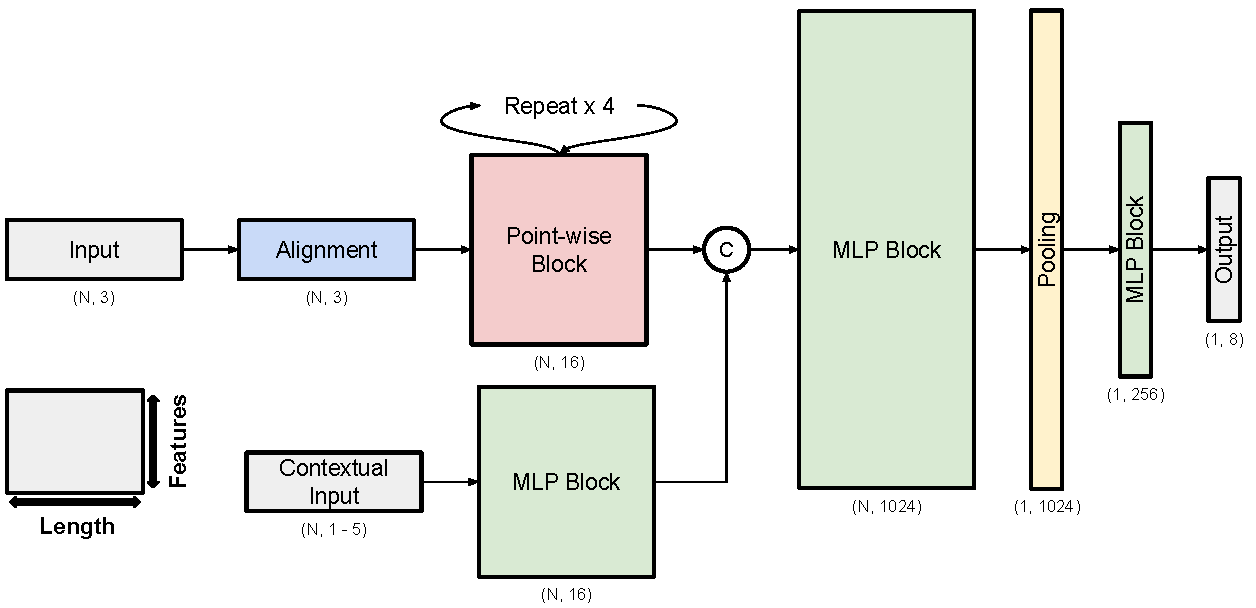
\includegraphics[width=1\textwidth]{figures/chapter4/PointFISH_architecture}
    \caption{PointFISH architecture template}
    \label{fig:PointFISH_architecture}
\end{figure}

\begin{figure}[h]
    \centering
    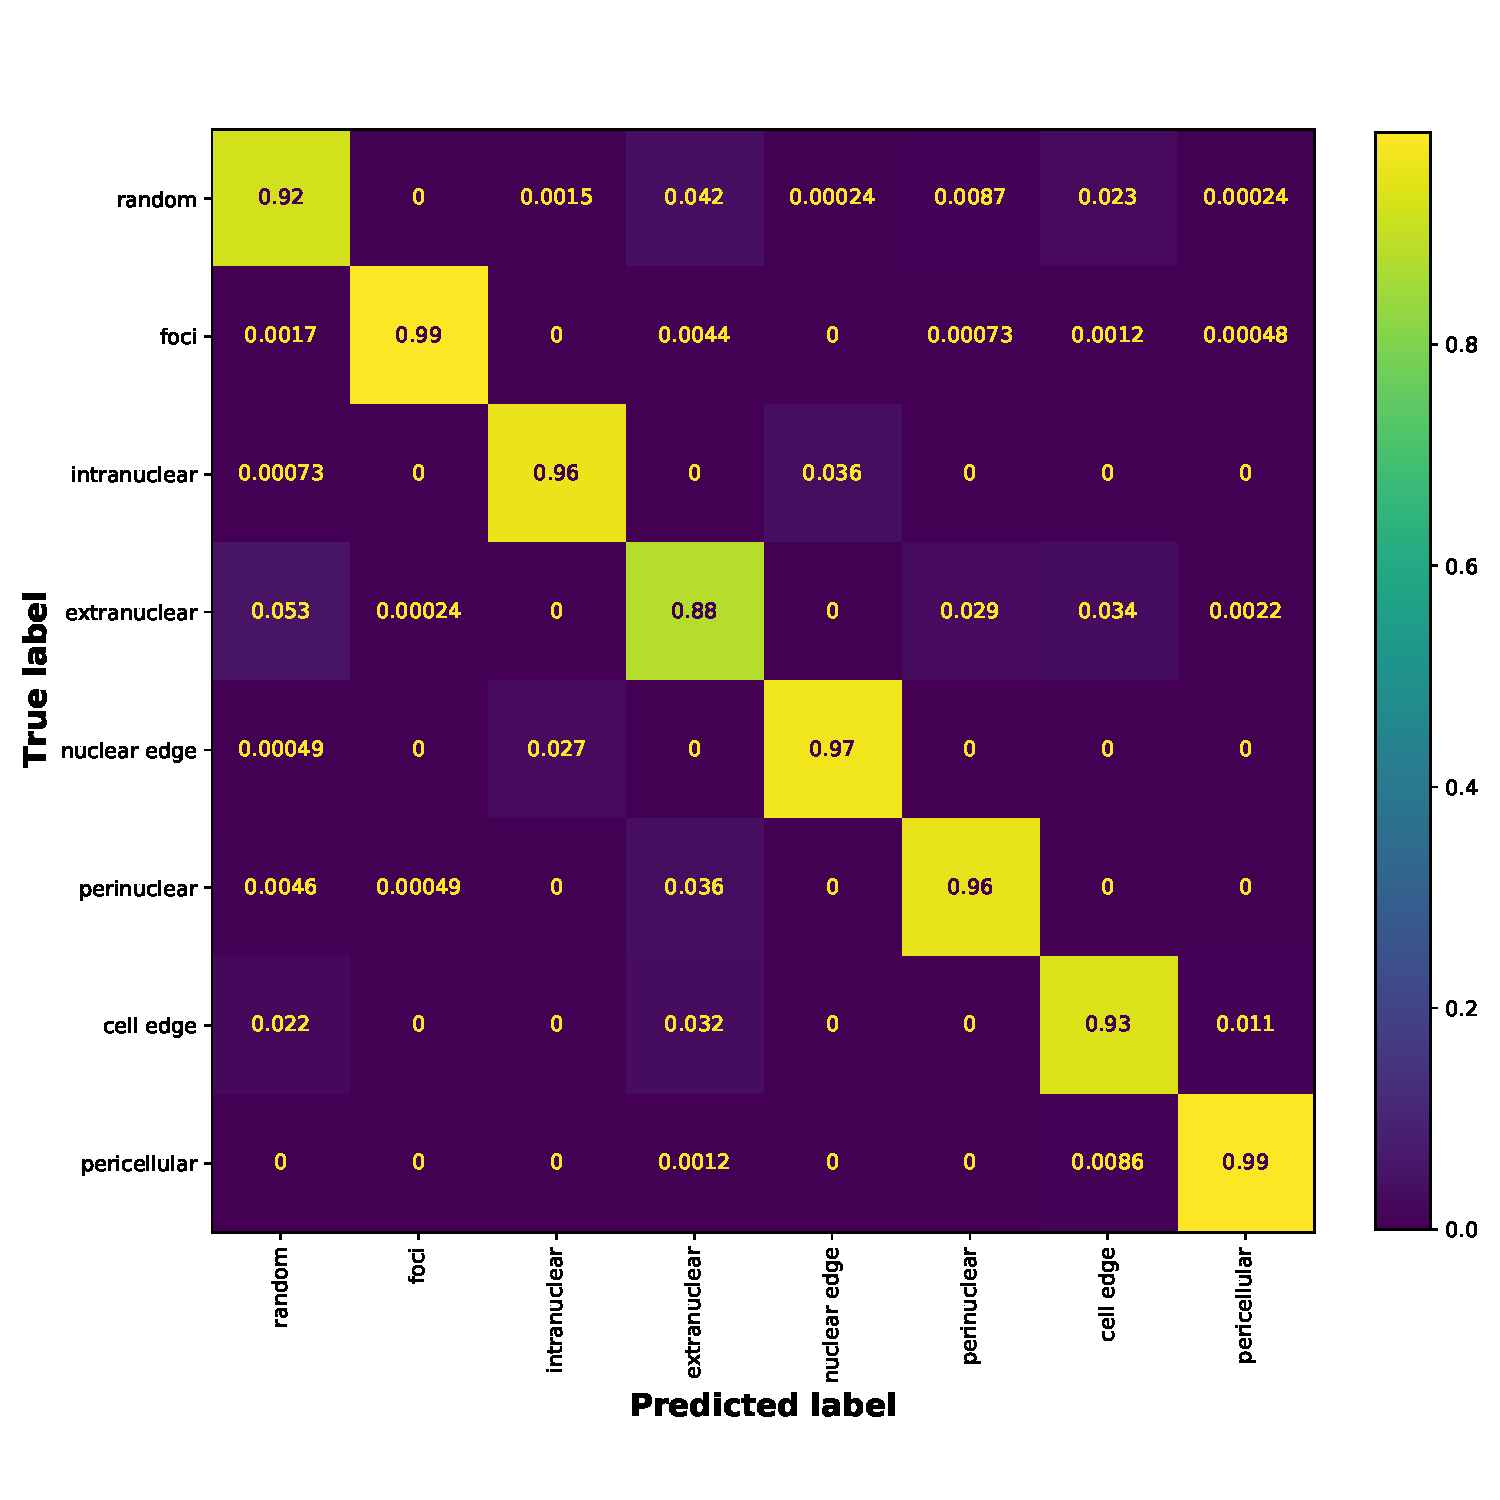
\includegraphics[width=0.7\textwidth]{figures/chapter4/confusion_matrix}
    \caption{Confusion matrix with simulated patterns}
    \label{fig:confusion_matrix}
\end{figure}


\subsection{Embedding extraction} \label{subsec:learned_embedding}

% brief description of the real dataset
% results supervised
% plot boxplot
% results unsupervised
% plot umap
% (plot dendogram)

\begin{figure}[h]
    \centering
    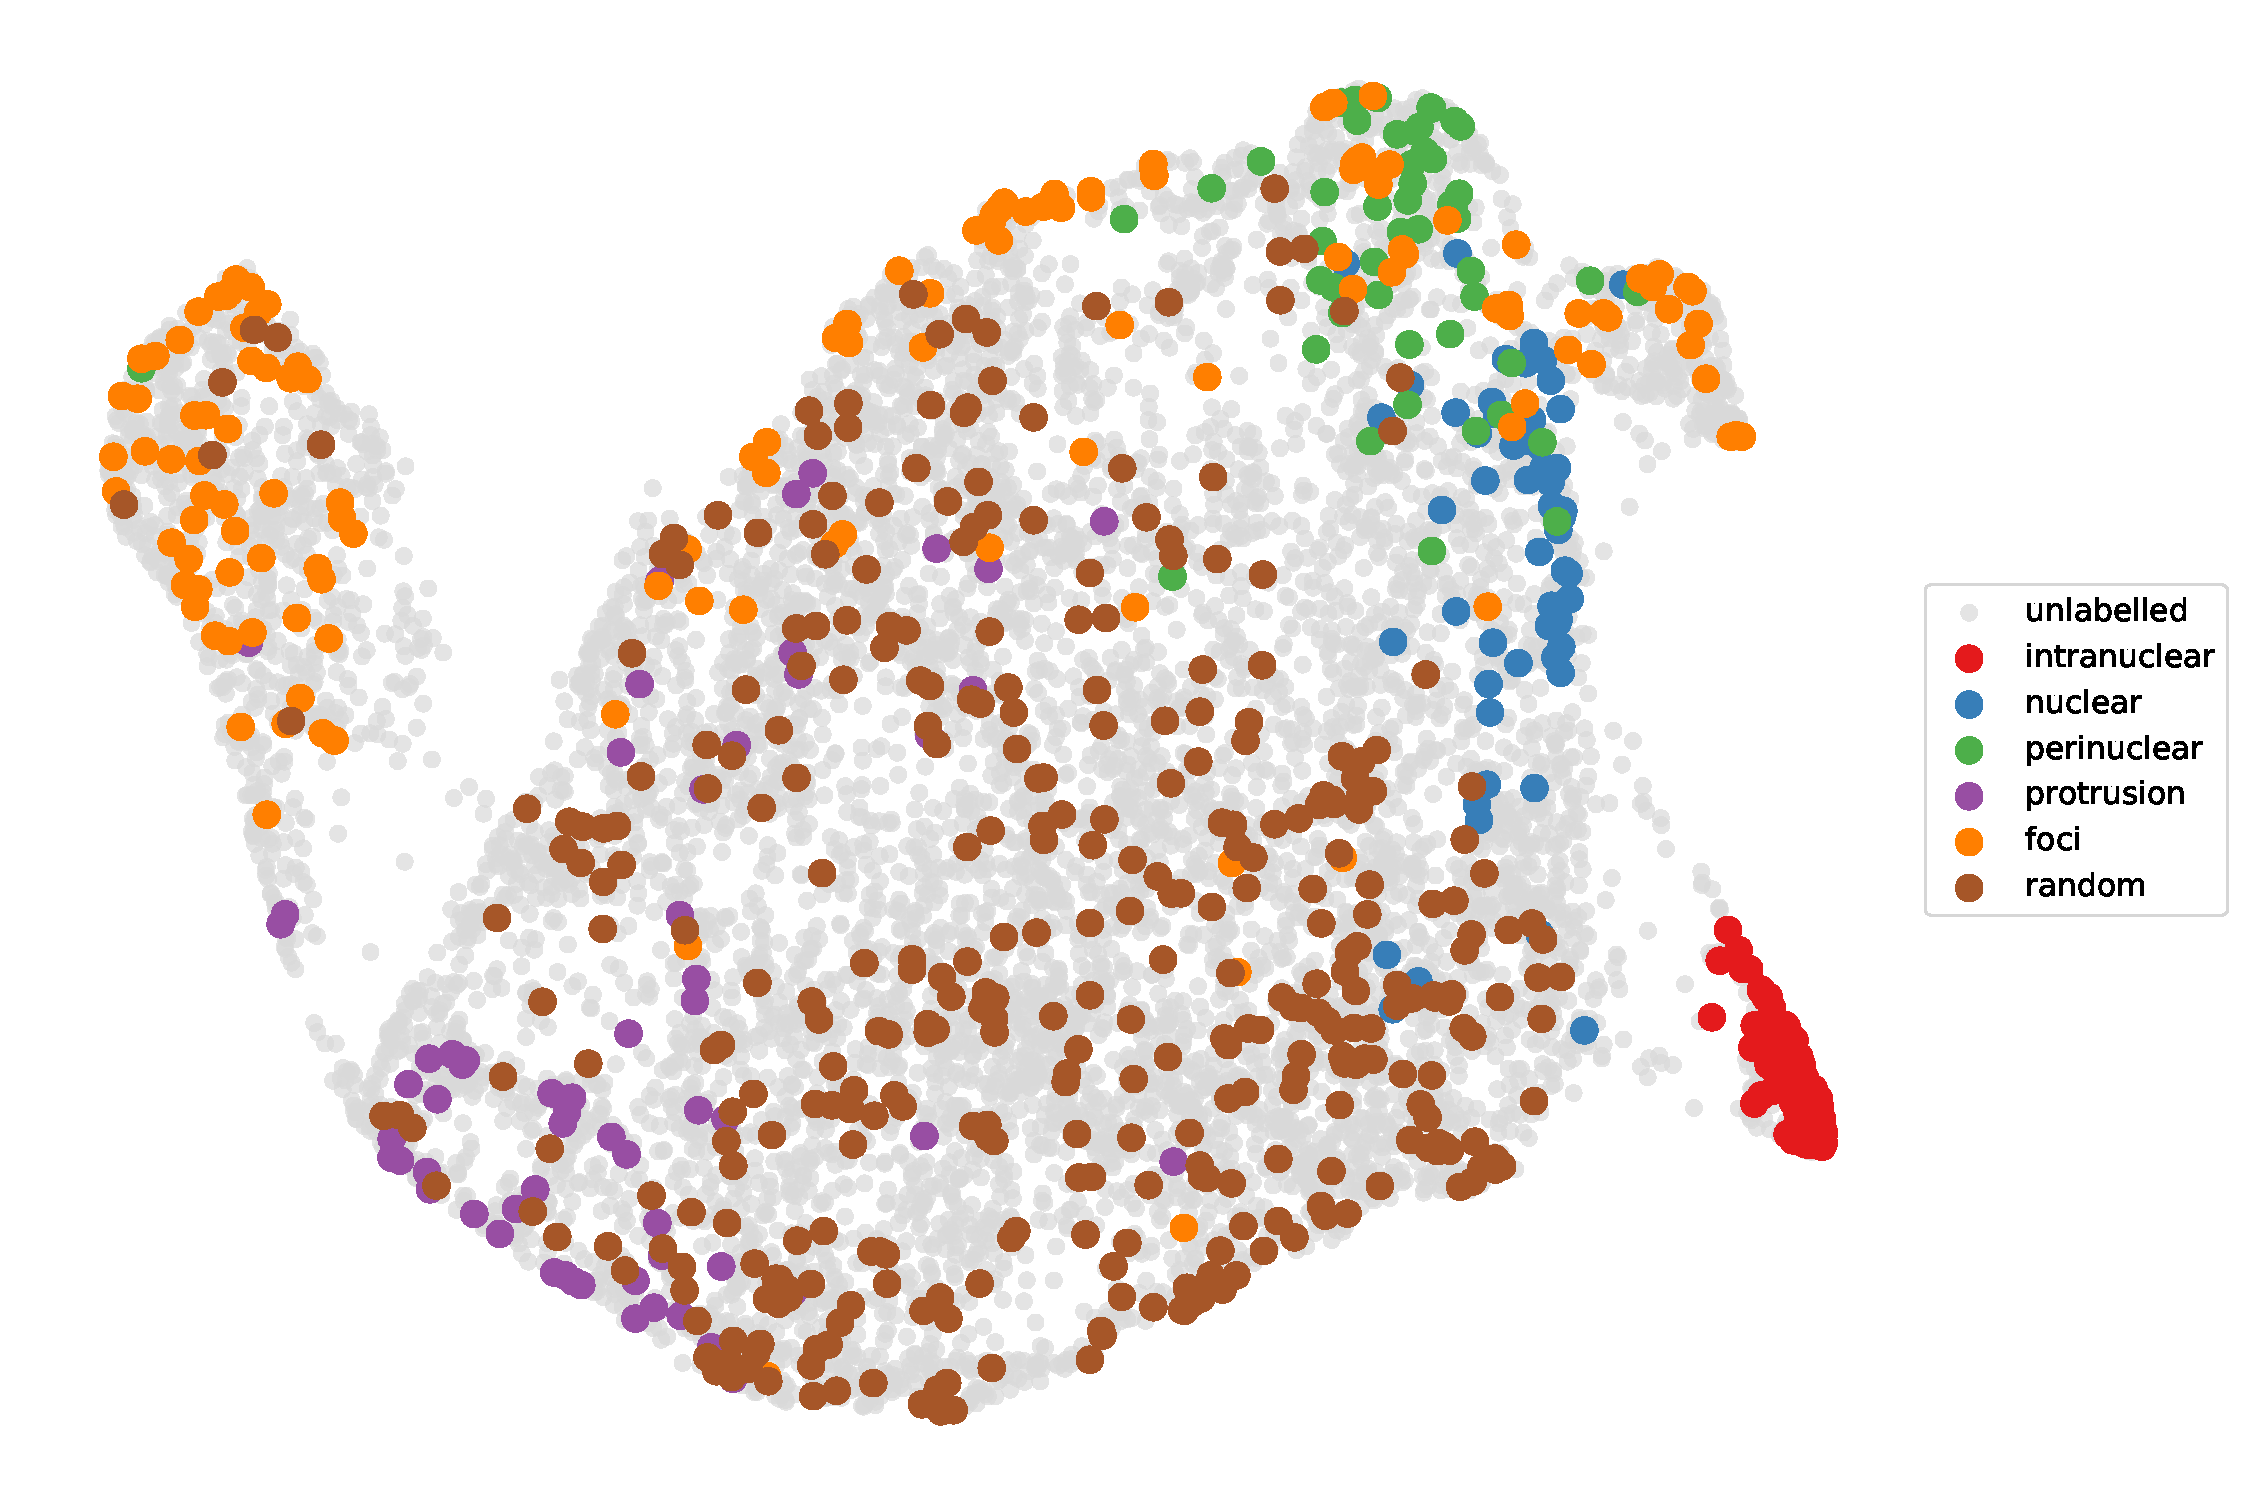
\includegraphics[width=1\textwidth]{figures/chapter4/umap_real}
    \caption{UMAP embedding with learned features}
    \label{fig:umap_real}
\end{figure}

\begin{figure}[h]
    \centering
    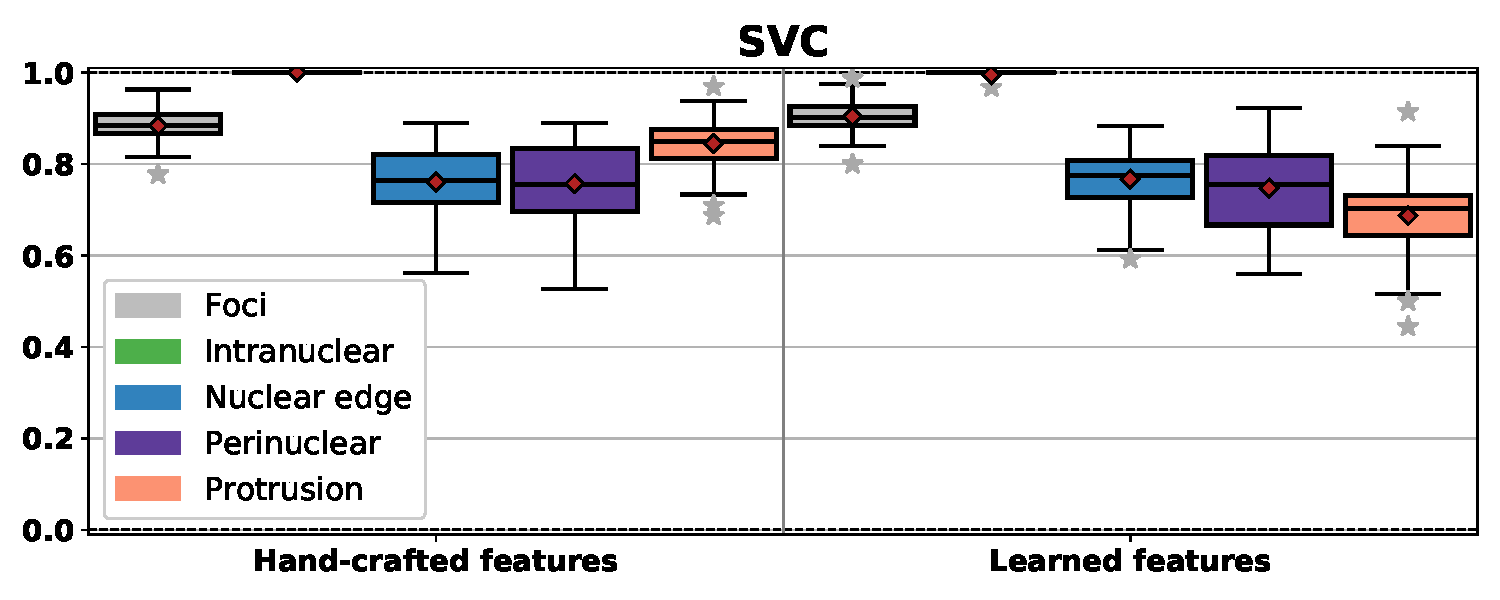
\includegraphics[width=1\textwidth]{figures/chapter4/f1_SVC}
    \caption{F1-score with localization pattern classification (SVC model)}
    \label{fig:f1_SVC_real}
\end{figure}


\section{Conclusion} \label{sec:analysis_conclusion}

% learned features from convnet
% from features engineering to simulation engineering